\section{CPU-level Energy Measurements}

High quality instruction level energy models can be derived for pipelined
processors by monitoring the instantaneous current drawn by the processor at
each clock cycle \cite{nikolaidis2005instruction}. As modern processors commonly
operate at a few GHz, expensive measurement devices are required to sample
at sufficient frequency.



\begin{figure}
    \centering
    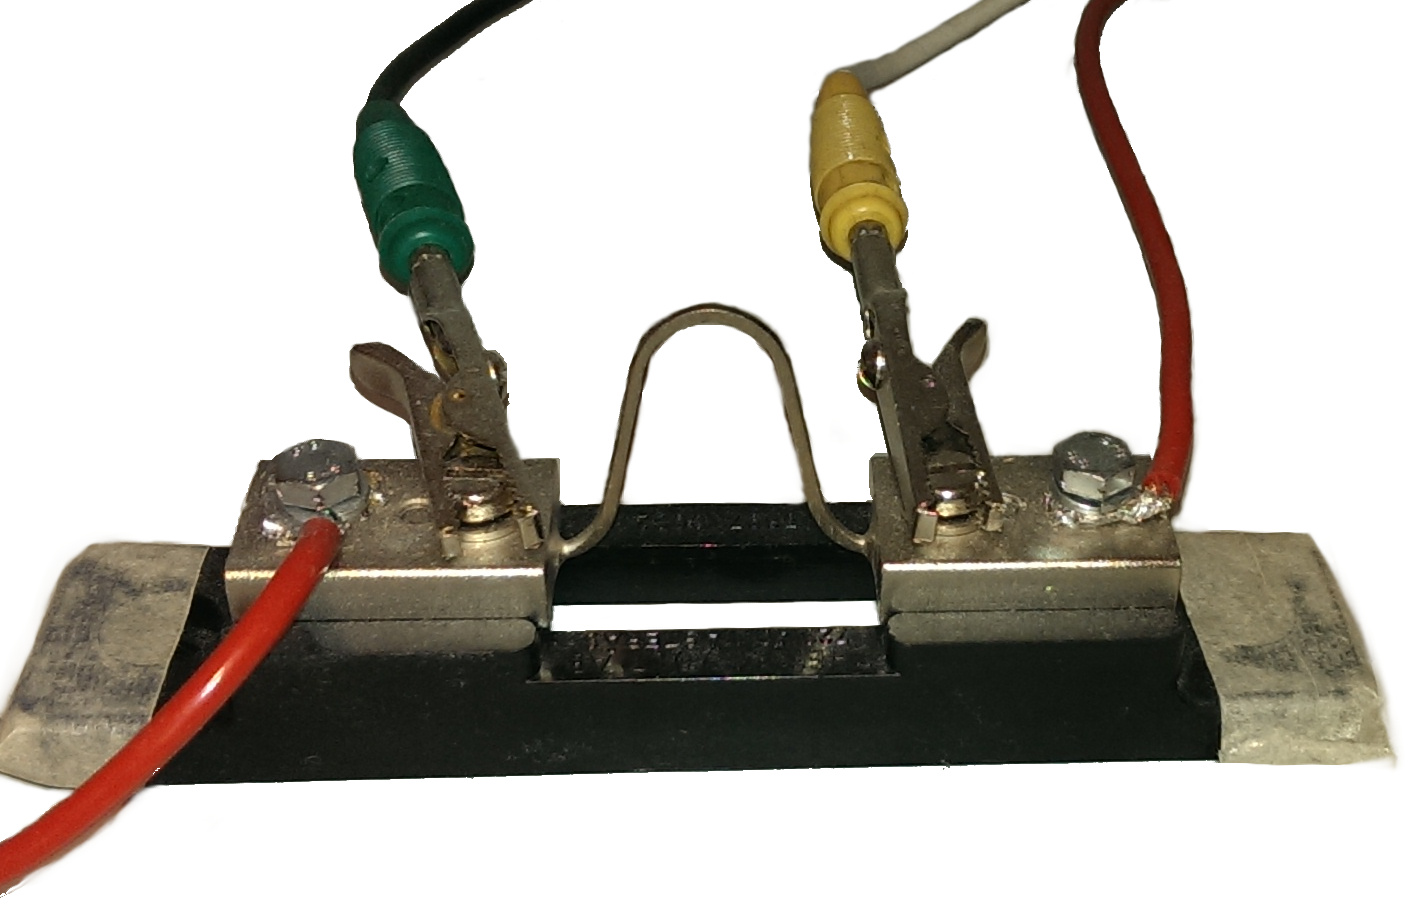
\includegraphics[width=0.8\textwidth]{figs/shunt.jpg}
    \caption{An example shunt resistor}
    \label{fig:shunt}
\end{figure}

% TODO: Where does this fit?
% The ultimate goal in this context is to estimate power consumption and energy
% efficiency of new hardware, the first step is to measure different more or less
% power consuming events on real hardware that is similar to the one simulated.

